\section{Source-level Debugging of Optimized Code}
A {\em source-level} (or {\em symbolic}) {\em debugger} is a program development tool that allows a programmer to monitor an executing program at the source-language level. Interactive mechanisms are typically provided to the user to halt/resume the execution at {\em breakpoints}, and to inspect the state of the program in terms of its source language. The importance of the design and use of these tools was already clear in the '60s~\cite{Evans66}.

\missing % DIRE DEI MOTIVI (vedi tesi Adl etc) - DEVO DIRE ANCHE LA COSA DI SINK E DCE?

As pointed out by Hennessy in his seminal paper from 1982~\cite{Hennessy82}, a classic conflict exists between the application of optimization techniques and the ability to debug a program symbolically. A debugger provides the user with the illusion that the source program is executing one statement at a time. On the other hand, optimizations preserve the semantic equivalence between optimized and unoptimized code, but normally alter the structure or intermediate results of a program.

Two problems surface when trying to symbolically debug optimized code~\cite{Adl-Tabatabai96,Jaramillo00}. First, the debugger must determine the position in the optimized code that corresponds to the breakpoint in the source code ({\em code location} problem). Second, the user expects to see the values of source variables at a breakpoint in a manner consistent with the source code, even though the optimizer might have 
deleted or reordered instructions, or values might have been overwritten as a consequence of the register allocator's choices ({\em data location} problem).

In general, there are two ways for a symbolic debugger to present meaningful information about the debugged optimized program~\cite{Wu99}. It provides {\em expected behavior} of the program if it hides the effect of the optimizations from the user and presents the program state consistent with what the user expects from the unoptimized code. It provides {\em truthful behavior} if it makes the user aware of the effects of optimizations and warns of possibly surprising outcomes.

Adl-Tabatabai observes in his PhD thesis that constraining optimizations or adding machinery during compilation to aid debugging do not solve the problem of debugging the optimized translation of a program, as the user debugs suboptimal code~\cite{Adl-Tabatabai96thesis}. Source-level debuggers thus need to implement techniques to recover expected behavior when possible, without relying on intrusive compiler extensions.

\subsection{Using \texorpdfstring{$\texttt{build\_comp}$}{build\_comp} for State Recovery}
%\subsection{Using  for State Recovery}
On-Stack Replacement has been pioneered in implementations of the SELF programming language to provide expected behavior with globally optimized code~\cite{Holzle92}. OSR shields the debugger from the effects of optimizations by dynamically deoptimizing code on demand. Debugging information is supplied by the compiler at discrete {\em interrupt points}, which act as a barrier for optimizations, letting the compiler run unhindered between them. Starting from the observation that our algorithms for generating OSR mappings (\mysection\ref{ss:osr-mapping}) do not place barriers for live-variable equivalent transformations, we investigated whether they could encode useful information for expected-behavior recovery in a source-level debugger.

As in most recent works on optimized code debugging, we focus on identifying and recovering scalar source variables in the presence of global optimizations. In LLVM, debugging information is inserted by the front-end as {\em metadata} attached to global variables, single instructions, functions or entire IR modules. Debugging metadata are transparent to optimization passes, do not prevent optimizations from happening, and are designed to be agnostic about the target debugging information representation (e.g., DWARF, stabs). Two intrinsics are used to associate IR virtual registers with source-level variables:
\begin{itemize}[itemsep=0pt,parsep=3pt]
 \item \mytt{llvm.dbg.declare} typically associates a source variable with an \alloca\footnote{\alloca\ is used to allocate space on the stack of the current function, to be automatically released when the function returns. Front-ends are not required to generate code in SSA form, but they can manipulate local variables created with \alloca\ using \load\ and \store\ instruction. Then the SSA form can be constructed using \memtoreg.} buffer;
 \item \mytt{llvm.dbg.value} informs that a source variable is being set to the value held by the virtual register.
\end{itemize}

\noindent We extended \tinyvm\ to reconstruct this mapping and also to indentify which program locations in the unoptimized IR version $f_{base}$ correspond to source-level locations for a function (as they would correspond to a possible user breakpoint location). An OSR mapping is then generated when OSR-aware transformation passes are applied to $f_{base}$ to generate the optimized version $f_{opt}$. For each location in $f_{opt}$ that might correspond to (i.e., have as OSR landing pad) a source-level location in $f_{base}$, we determine which variables live at destination are live also at source (and thus yield the same value), and which instead need to be reconstructed. We thus rely on the SSA form to identify which assignment(s) should be made in \reconstruct, as distinct assignments to source-level variables are represented by distinct IR objects. $\phi$-nodes at control-flow merge points of course can not be reconstructed, but our preliminary experimental investigation suggests that this might not be a huge issue in practice.

\missing % DIRE DI COME USARE QUESTE INFO (invisible breakpoints lo dico dopo?)

%As pointed out in~\cite{Adl-Tabatabai96}, compiler transformations cause {\em endangered} variables by either eliminating or moving assignments to source variables. 

\subsection{Experimental Results}
To capture a variety of programming patterns and styles from applications with different sizes, we have analyzed each method for each C benchmark in the \speccpu\ suite.

\begin{table}[ht]
\begin{center}
\begin{small}
\begin{tabular}{ |c|r|r|r|r|r|r|r| }
\cline{3-8}
\multicolumn{2}{l|}{} & \multicolumn{6}{c|}{Functions} \\
\cline{3-8}
\multicolumn{2}{l|}{} & \multicolumn{1}{c|}{Total} & \multicolumn{2}{c|}{Optimized} & \multicolumn{3}{c|}{Endangered} \\
\hline
Benchmark & \multicolumn{1}{c|}{LOC} & \multicolumn{1}{c|}{$f_{tot}$} & \multicolumn{1}{c|}{$f_{opt}$}  & \multicolumn{1}{c|}{\unitfrac{$f_{opt}$}{$f_{tot}$}} & \multicolumn{1}{c|}{$f_{end}$} & \multicolumn{1}{c|}{\unitfrac{$f_{end}$}{$f_{tot}$}} & \multicolumn{1}{c|}{\unitfrac{$f_{opt}$}{$f_{opt}$}} \\ 
\hline
\hline
bzip2 & 8\,293 & 100 & 66 & 0.66 & 24 & 0.24 & 0.36 \\ 
\hline
gcc & 521\,078 & 5\,577 & 3\,884 & 0.70 & 1\,149 & 0.21 & 0.30 \\
\hline
gobmk & 197\,215 & 2\,523 & 1\,664 & 0.66 & 893 & 0.35 & 0.54 \\ 
\hline
h264ref & 51\,578 & 590 & 466 & 0.79 & 163 & 0.28 & 0.35 \\ 
\hline
hmmer & 35\,992 & 538 & 429 & 0.80 & 80 & 0.15 & 0.19 \\ 
\hline
lbm & 1\,155 & 19 & 17 & 0.89 & 2 & 0.11 & 0.12 \\ 
\hline
libquantum & 4\,358 & 115 & 85 & 0.74 & 9 & 0.08 & 0.11\\ 
\hline
mcf & 2\,658 & 24 & 21 & 0.88 & 11 & 0.46 & 0.52 \\ 
\hline
milc & 15\,042 & 235 & 157 & 0.67 & 34 & 0.14 & 0.22\\ 
\hline
perlbench & 155\,418 & 1\,870 & 1\,286 & 0.69 & 593 & 0.32 & 0.46 \\ 
\hline
sjeng & 13\,847 & 144 & 113 & 0.78 & 31 & 0.22 & 0.27 \\ 
\hline
sphinx3 & 25\,090 & 369 & 275 & 0.75 & 76 & 0.21 & 0.28 \\ 
\hline
\end{tabular} 
\end{small}
\end{center}
\caption{\label{tab:CS-debug-benchmarks} Description of the C benchmarks in the \speccpu\ suite.} 
\end{table}

\begin{figure}[!ht]
\begin{center}
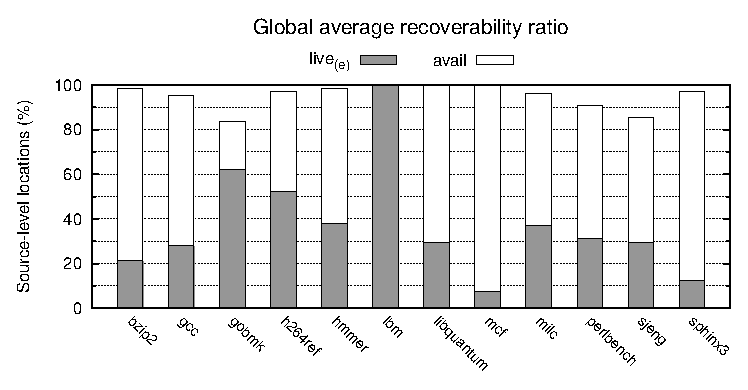
\includegraphics[width=0.8\textwidth]{figures/CS-debug-ratio/CS-debug-ratio.eps}
\caption{\protect\label{fig:CS-debug-ratio} Global average recoverability ratio, defined as weighted average of each function's average recoverability ratio. We used the number of LLVM IR instructions in the unoptimized function version as weight.}
\end{center}
\end{figure}


%However, when attempting to debug optimized programs, most debuggers may give misleading information about the value of variables at breakpoints.
%Hence, the programmer has the difficult task of attempting to unravel the optimized code 